% Sample file on how to use subfiles.
\documentclass[ExampleMasters.tex]{subfiles}

\begin{document}
\clearpage
{\pagestyle{empty}\cleardoublepage}%
\chapter{Vehicle Model controllers}
\label{chap:steering_model}
The vehicle model controllers that were used in this thesis were developed in a research project at Chalmers.
There are two different controllers used to control the steerable axles of the dolly. One is used for low-speed and one for high-speed maneuvers. The main purpose of the low-speed controller is the reduction of off-tracking.
For the high-speed controller the aim is to reduce the rearward amplification.
\section[Low-Speed controller]{Low-Speed controller \cite{Low-speed_paper}}
\label{sec:low-speed_controller}
The low-speed controller is implemented in path-distance domain $\eta$. The path-distance is calculated by integrating the forward speed $v_{x,1}(t)$. \\
The steering angle of the first axle of the dolly is calculated as follows: 
\begin{equation}
\delta_{31}(\eta)=k_1\delta_{11}(\eta-\eta_1)+k_2\Delta\psi_1(\eta-\eta_2)+k_3\Delta\psi_2(\eta-\eta_3)+k_4\Delta\psi_3(\eta-\eta_4)
\end{equation}
\label{eq:delta31_lowspeed}
where $\delta_{31}$ is the steering angle of the dolly's front axle, $\delta_{11}$ is the steering angle of the tractor's front axle, $\Delta\psi_1$ the articulation angle between the tractor and the first semitrailer, $\Delta\psi_2$ the articulation angle between the first semitrailer and the dolly, $\Delta\psi_3$ the articulation angle between the dolly and the second semitrailer, $\eta_1$ the distance between the tractor's first axle and the dolly's first axle, $\eta_2$ the distance between the first articulation joint and the dolly's first axle, $\eta_3$ the distance between the second articulation joint and the dolly's first axle, $\eta_4$ the distance between the third articulation joint and the dolly's first axle, and $k_1, k_2, k_3, k_4$ are gains. 
\\The steering angle of the second axle of the dolly is calculated using the steering angle of the first dolly axle as follows:
\begin{equation}
\delta_{32}(\eta)=k_5\delta_{31}(\eta-\eta_5)
\end{equation}
\label{eq:delta32_lowspeed}
where $\delta_{32}$ is the steering angle of the dolly's second axle, $\eta_5$ is the distance between the dolly's second and first axle, and $k_5$ is a gain.\\
The gains $k_1, k_2, k_3, k_4, k_5$ were optimized using the particle swarm optimization.
Table \ref{tab:gains_after_optimization} shows the values of the gains after the optimization and the improvement of the controller for different maneuvers compared to a simulation without steering of the dolly.
\begin{table}[h]
	\centering
	\caption{Control gains and performance improvement}
	\label{tab:gains_after_optimization}
	\begin{tabular}{l|l|l l l}
		& &  & Improvement  \\ \hline
		Gain & Value & 180-deg turn (\%) & 90-deg turn (\%) & S-turn\\ \hline
		$k_1$   &       -0.2126      &             \\
		$k_2$    &            -0.1567 &             \\
		$k_3$  &      -0.8780       &           +44.61 & +37.75 & +45.07  \\
		$k_4$ &      -0.3143       &           \\
		$k_5$  & 0.9868 & \\
		
	\end{tabular} \\
\end{table}\\
Figure \ref{fig:low_speed_diagram} shows the implementation of the controller in the functional architecture, introduced in section \ref{sec:func_architecture}.

\begin{figure*}[!htb]
	\centering
	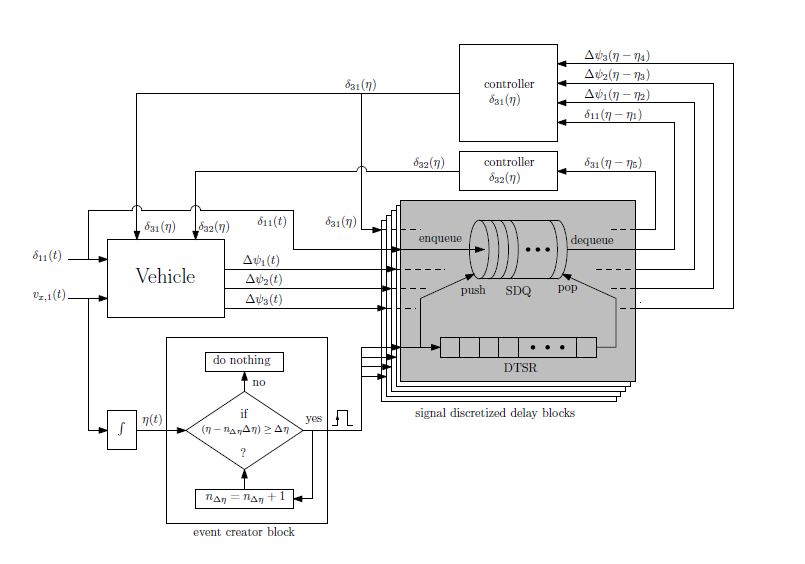
\includegraphics[width=1.0\linewidth]{figures/Low_speed_diagram}
	\caption[Controller implementation in the functionality architecture]{Controller implementation in the functionality architecture \cite{Low-speed_paper}}
	\label{fig:low_speed_diagram}
\end{figure*}

\subsection{Input parameters}
\label{sec:input_parameters_LS}
The input parameters for the low-speed controller are:
\begin{itemize}
	\item The articulation angles between the different units: $\Delta\psi_1$, $\Delta\psi_2$, $\Delta\psi_3$
	\item The steering angle of the tractor's first axle: $\delta_{11}$
	\item The distances of the tractor's first axle, the articulation joints of the different units and the dolly's second axle to the dolly's first axle: $\eta_1,\eta_2,\eta_3,\eta_4,\eta_5$
	\item The vehicle speed for the transformation from time to path-distance domain:  $v_x$
	
\end{itemize}

\section[High-Speed controller]{High-Speed controller \cite{High-speed_paper}}
\label{sec:high-speed_controller}
The high-speed controller is implemented using a nonlinear inverse of a dynamic vehicle model.
The aim of the controller is to copy the movement of the first unit to the following ones at a certain point. Therefore the movements of the following units need to be delayed by the time it takes them to reach this point. For the dolly unit, this delay $\tau_{13}$ is calculated with the vehicle speed $v_x$ and the distance $l_{cg13}$ between the \gls{COG}  of the tractor and the dolly as follows:
\begin{equation}
\tau_{13}=\frac{l_{cg13}}{v_x(t)}
\end{equation}
With this delay and the lateral acceleration of the tractor $a_{y1}$ a reference signal for the dolly's lateral acceleration is calculated as follows:
\begin{equation}
a_{y3ref}(t)=a_{y1}(t-\tau_{13})
\end{equation}
This reference signal, together with the steering angle of the tractor, the forward speed of the vehicle and the actual steering angle of the dolly, is used as inputs to an inverse single track model, that is modeled in the Modelica language. The outputs of the model are the request steering angle $\delta_{dolreq}$ and the lateral acceleration $a_{y3}$ of the dolly. Figure \ref{fig:inverse_single_track_model} shows a block diagram of that model.  

\begin{figure*}[!htb]
	\centering
	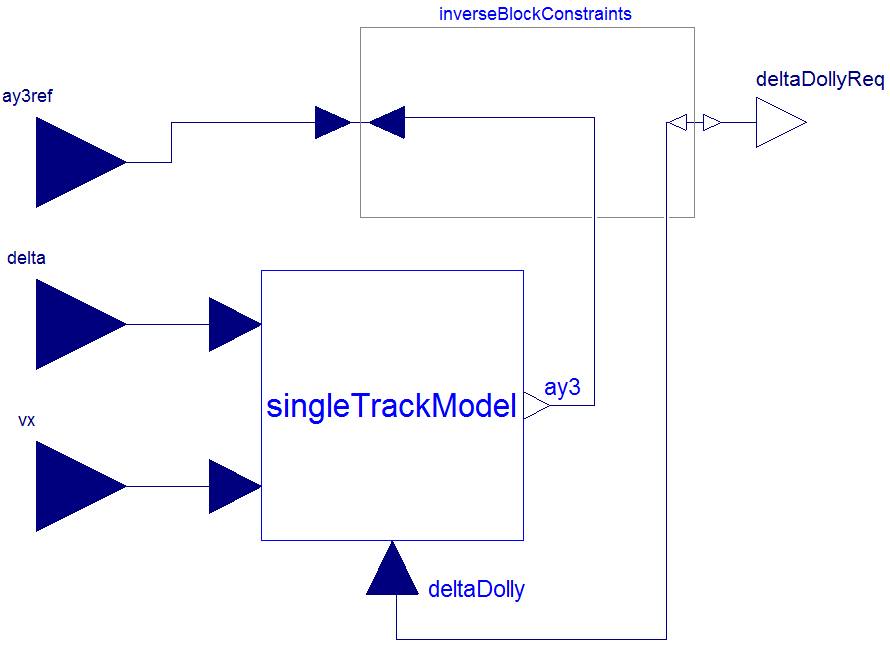
\includegraphics[width=0.5\linewidth]{figures/Inverse_of_A-double_single-track}
	\caption[Inverse of the single track A-double model]{Inverse of the single track A-double model \cite{High-speed_paper}}
	
	\label{fig:inverse_single_track_model}
\end{figure*}

To determine the performance of this controller simulations of a single lane change at 20 meters per second and a sine wave steering input of 0.4 Hz with an amplitude of 0.026 rad were done. As a result the rearward amplification of the yaw rate of the second trailer is 0.95 with this controller compared to 1.49 for a passive dolly. Furthermore the transient off-tracking is improved by 67\%. 

\subsection{Input parameters}
\label{sec:input_parameters_HS}
Figure \ref{fig:inverse_model_controller} shows the input and outputs of the inverse model controller.
\begin{figure*}[!htb]
	\centering
	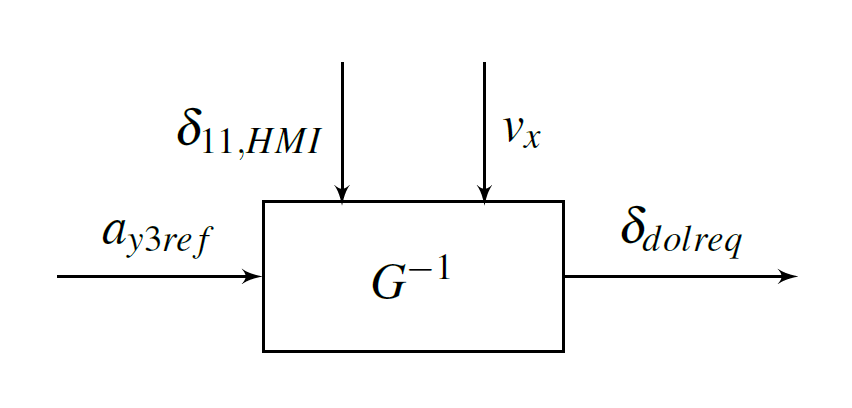
\includegraphics[width=0.5\linewidth]{figures/inverse_controller}
	\caption[Inverse model controller]{Inverse model controller\cite{High-speed_paper}}
	
	\label{fig:inverse_model_controller}
\end{figure*}\\
The input parameters of the high-speed controller are:
\begin{itemize}
\item The vehicle speed: $v_x$ 
\item The steering angle of the tractor's front axle: $\delta_{11}$
\item The reference signal of the lateral acceleration of the dolly: $a_{y3ref}$
\end{itemize}


\section{Interface with Real-Time environment}
\label{sec:interface_with_real_time}
As described in section \ref{sec:low-speed_controller} and \ref{sec:high-speed_controller} the controllers need different kind of input signals. These signals are received by the Simulink model running on the \gls{MABII} via \gls{CAN} (refer to section \ref{sec:matlab}). When the controllers are tested on a test track they are implemented in the same Simulink model, so they can get the necessary input signals directly within the model. For the \gls{HIL}-tests, that were conducted the controllers where implemented in a Simulink model running on a simulation PC. In that case the necessary inputs were sent to this PC via serial interface. In  section \ref{sec:HIL} this approach is described in detail.     

In order to guaranty safety at all time the steering angle requests of the controllers are checked before sending them to the dolly. This is done by first sending the requests to a supervisor block in the same Simulink model. The supervisor block compares the steering angle requests with the current capabilities of the system. The functionality of that block is described in detail in section \ref{sec:warning_system}.   



\end{document}
